\documentclass[conference]{IEEEtran}
\IEEEoverridecommandlockouts

% ==== Fuente moderna (compatible XeLaTeX + Windows) ====
\usepackage{fontspec}
\setmainfont{Times New Roman}
\usepackage{newtxmath}

% ==== Custom Abstract & Keywords ====
\makeatletter
\newenvironment{customabstract}{
  \vspace{1em}
  \noindent{\emph{\textbf{Abstract —}}}\hspace{0.5em}\textbf
}{\par\vspace{1em}}

\newenvironment{customkeywords}{
  \vspace{0.5em}
  \noindent{\emph{\textbf{Keywords -}}}\hspace{0.5em}\itshape
}{\par\vspace{1em}}
\makeatother

\usepackage{graphicx}
\usepackage{cite}
\usepackage{amsmath}
\usepackage{url}
\usepackage{hyperref}

\begin{document}

\title{Intelligent Online Notification Manager Using Machine Learning for the Standardization of Messaging Services in the Private Banking Sector}

% === Two-column authors ===
\author{
  {\small
    \begin{minipage}[t]{0.45\textwidth}
      \centering
      \textbf{Wilmer Andres Quispe Gomez}\\
      Faculty of Engineering\\
      Universidad Peruana de Ciencias Aplicadas (UPC)\\
      Lima, Peru\\
      \texttt{u202324341@upc.edu.pe}
    \end{minipage}
    \hfill
    \begin{minipage}[t]{0.45\textwidth}
      \centering
      \textbf{Moises Jhonatan Lagos Pachas}\\
      Faculty of Engineering\\
      Universidad Peruana de Ciencias Aplicadas (UPC)\\
      Lima, Peru\\
      \texttt{u20171a978@upc.edu.pe}
    \end{minipage}
  }
}

\maketitle

\begin{customabstract}
This paper presents the design of an intelligent online notification manager that leverages machine learning (ML) to unify and optimize the delivery of digital notifications across multiple communication services in the private banking sector. The system proposes a microservices-based architecture integrated with a scalable Application Programming Interface (API) to homogenize channels such as email, SMS, push notifications, and WhatsApp. By applying reinforcement learning and supervised classification models, the system determines the optimal channel, timing, and message content for each user. The implementation ensures compliance with Peruvian regulatory standards (Law No. 29733, SBS Resolution No. 504-2021) and international security standards (ISO/IEC 27001). This work contributes to the modernization of communication systems in financial institutions by improving customer experience, operational efficiency, and traceability.
\end{customabstract}

\begin{customkeywords}
machine learning; multi-channel messaging; API; financial technology; notification system
\end{customkeywords}

\section{Introduction}

In the current digital era, financial institutions face increasing pressure to deliver consistent, secure, and personalized communication experiences to their clients across multiple channels. In the private banking sector, this challenge is intensified by the coexistence of heterogeneous notification services—such as Firebase, APNs, email, and SMS—which often operate in isolation and lead to fragmentation, duplicated efforts, and higher operational costs \cite{alzahrani2020}. This paper addresses this problem by proposing an intelligent online notification manager powered by machine learning to unify and optimize message delivery through a scalable and secure API.

The problem is interesting and relevant because notification systems represent a critical interface between banks and clients. According to Twilio \cite{twilio2023}, 98\% of customers expect consistent communication experiences across all channels. However, existing platforms such as OneSignal, Airship, or Amazon SNS lack adaptive intelligence capable of learning user behavior, predicting optimal delivery moments, or dynamically selecting the most effective channel. These limitations prevent financial institutions from achieving true omnichannel consistency and operational efficiency.

The problem is difficult to solve because naive approaches to multichannel messaging rely on static rules and manual configurations that do not adapt to the user’s context or response patterns. Moreover, the banking environment imposes additional constraints—such as strict regulatory compliance (e.g., SBS Resolution No. 504-2021) and data confidentiality—that make integration and automation even more challenging.

Previous solutions have focused primarily on technical integration, ignoring intelligent decision-making. While some frameworks like the Integrated Multi-channel Messaging Model (IM3) \cite{liang2011} provide a structural foundation for message transformation and routing, they do not incorporate learning algorithms to optimize communication flow. Other studies demonstrate that applying machine learning to notifications can significantly improve engagement and response rates \cite{rahimi2021}, yet these solutions have not been adapted to the requirements of the financial sector.

Our contribution lies in developing and validating an intelligent notification management model that combines reinforcement learning and predictive analytics to determine the optimal channel, timing, and content of each message. The proposed system seeks to (1) unify existing communication services through an API-based architecture, (2) optimize message delivery through adaptive learning, and (3) ensure regulatory compliance and security required by the financial industry. Although our initial prototype focuses on the BBVA case study in Peru, the conceptual model is extensible to other financial institutions facing similar interoperability and personalization challenges.

This paper is structured as follows: Section II presents the theoretical background and related work. Section III describes the methodological framework and data sources. Section IV introduces the proposed model and architecture. Section V discusses the results and validation of the system, and Section VI presents conclusions and future research directions.

\section{State of the Art}

Different studies have explored how artificial intelligence and machine learning can enhance the effectiveness of multichannel communication systems, particularly in sectors requiring high personalization and regulatory compliance such as banking. This section provides a concise literature review comparing relevant approaches and highlighting how our work extends existing knowledge.

Salami and Mnkandla \cite{salami2022} proposed a \textit{Machine-Learning-Enabled Multi-Channel Messaging Framework} for financial institutions. Their architecture integrates an Enterprise Service Bus (ESB) with a machine learning module that selects the optimal communication channel based on previous user interactions. Although this framework demonstrates the feasibility of intelligent channel selection, it does not include reinforcement learning or real-time adaptation mechanisms. Our proposal builds on their approach by incorporating an adaptive learning model that continuously updates channel selection policies according to user feedback.

Similarly, Yancey and Settles \cite{yancey2020} developed the \textit{Recovering Difference Softmax Algorithm} (RDSA), designed to optimize recurring notifications in large-scale systems such as Duolingo. Their algorithm increased daily user retention by dynamically balancing exploration and exploitation. While their model excels in content optimization, it does not address multi-channel message integration or compliance with financial regulations. Our work extends this idea by applying similar adaptive strategies to financial notification systems, considering channel diversity and data confidentiality constraints.

López and Guerrero \cite{lopez2020} proposed a conceptual framework for smart device-based notifications that emphasizes contextual delivery and user attention management across IoT devices. Their research confirms that distributing notifications across multiple devices can reduce user overload. However, the framework is conceptual and lacks machine learning implementation. Our work operationalizes this concept by using predictive analytics to determine the best device or channel for each notification event.

Prabhakar et al. \cite{prabhakar2022} introduced an \textit{Offline Reinforcement Learning} approach for optimizing notification sequences, demonstrating improved engagement and reduced user annoyance compared to fixed schedules. Their findings validate the potential of reinforcement learning for adaptive messaging, yet their model is trained on generic datasets and not tailored to high-security sectors like banking. In contrast, our proposal contextualizes reinforcement learning within a financial environment, ensuring compliance with standards such as the SBS Resolution No. 504-2021 for secure communication.

Finally, Nicolas-Plata et al. \cite{nicolas2024} presented a \textit{service mesh} architecture to integrate processing patterns into microservices applications, providing a flexible way to orchestrate distributed communication systems. While their work focuses on scalability and fault tolerance, it lacks an intelligent decision-making layer. Our solution integrates a similar service mesh infrastructure but enhances it with a machine learning engine capable of autonomous channel orchestration and failure recovery.

In summary, previous research provides valuable foundations in three main areas: (1) architectural frameworks for multichannel communication \cite{salami2022, nicolas2024}, (2) adaptive algorithms for content and timing optimization \cite{yancey2020, prabhakar2022}, and (3) conceptual models for contextual notifications \cite{lopez2020}. However, none of these works simultaneously address the unification, intelligent adaptation, and regulatory compliance required in the private banking sector. Therefore, our contribution extends existing knowledge by combining these elements into an integrated, learning-based notification management system that adapts in real time and ensures secure, compliant, and efficient communication across multiple channels.

\section{Contribution: General Conceptualization}

The proposed contribution consists of the design of an intelligent notification manager capable of unifying all communication channels used by private banks into a single architecture. This system addresses the problem of fragmented and uncoordinated message delivery by introducing a centralized model supported by machine learning and application programming interfaces (APIs). Its goal is to standardize communication processes while maintaining flexibility and regulatory compliance \cite{rahimi2021,torres2020}.

Figure~\ref{fig:liu2011} presents a general conceptual diagram of the proposed model. It shows how the system integrates three main layers: the data layer, the intelligence layer, and the communication layer. The data layer stores historical records of notifications, user behavior, and delivery outcomes. The intelligence layer contains the machine learning models that analyze patterns and determine the most appropriate channel, timing, and content for each user. Finally, the communication layer manages the sending and tracking of messages through multiple services such as email, SMS, push notifications, and instant messaging \cite{liang2011}.

This conceptualization contributes to the automation of notification processes in private banking by transforming manual and repetitive tasks into data-driven decisions. It also enhances traceability and transparency, since every message is logged, monitored, and evaluated. According to the SBS Resolution No. 504-2021 \cite{sbs2021} and ISO/IEC 27001 \cite{iso27001}, such mechanisms are essential for guaranteeing information security and compliance in digital financial systems. Therefore, the proposed model represents a practical framework that aligns technological innovation with security standards and customer-centric communication.

\begin{figure}[htbp]
  \centering
  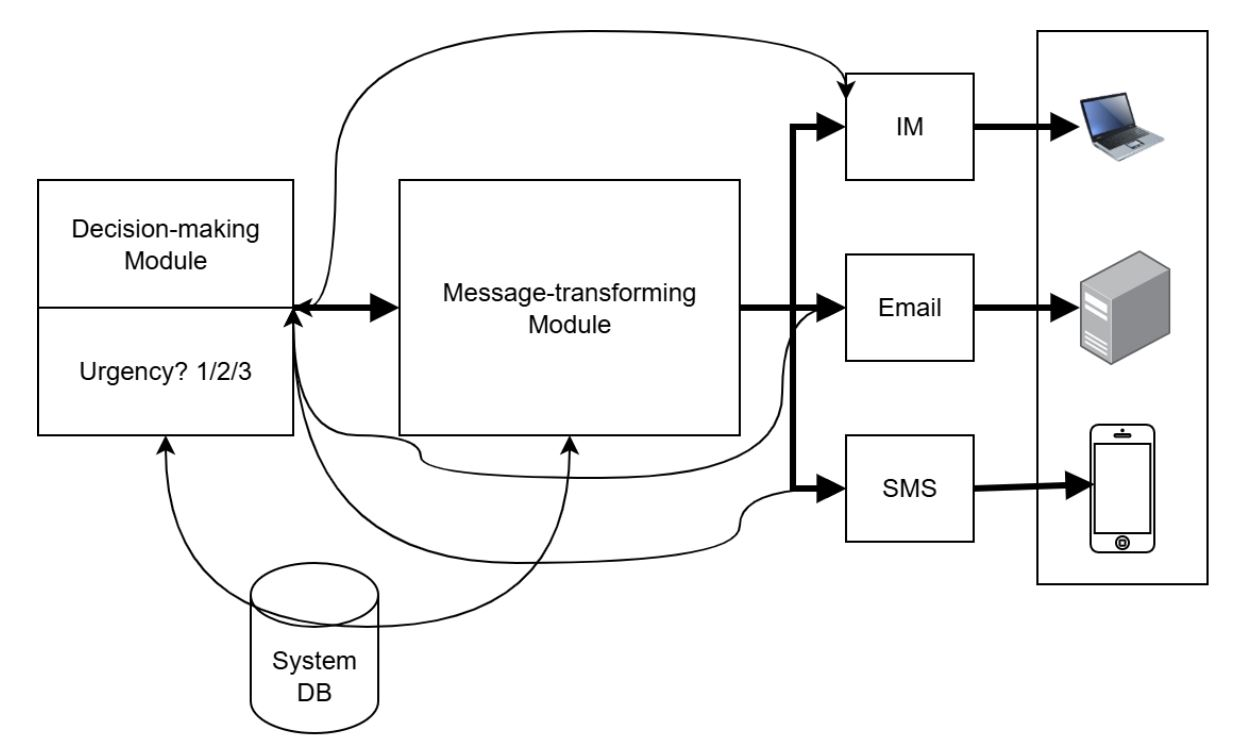
\includegraphics[width=0.45\textwidth]{liu2011-model.jpg}
  \caption{Integrated multi-channel messaging model supporting business collaboration \cite{liu2011}.}
  \label{fig:liu2011}
\end{figure}

\bibliographystyle{IEEEtran}
\bibliography{referencias}

\end{document}
